\documentclass[final,12pt]{article}    
%%%%%%%%%%%%%%%%%%%%%%%%%%%%%%%%%%%%%%%%%%%%%%%%%%%%%%%%%%%%%
%
%  include packages
%
\usepackage{times}
\usepackage{ifthen}
\usepackage{graphics}
\usepackage{color}
\usepackage{shadow}
%%%%%%%%%%%%%%%%%%%%%%%%%%%%%%%%%%%%%%%%%%%%%%%%%%%%%%%%%%%%%
%
%  if private=false certain descriptions are excluded using
%  the \ifthenelse expression
%
\newboolean{private}\setboolean{private}{true}
\newboolean{qmmm}\setboolean{qmmm}{true}
%%%%%%%%%%%%%%%%%%%%%%%%%%%%%%%%%%%%%%%%%%%%%%%%%%%%%%%%%%%%%
%
%  define commands
%
\newcommand{\block}[1]{\subsubsection[#1]{\shabox{\bf #1}}}
%
\newcommand{\brules}[1]{
\makebox[1in][l]{Rules:}\parbox[t]{110mm}{#1}\hfill\break\hfill}
%
\newcommand{\bdescr}[1]{
\makebox[1in][l]{Description:}\parbox[t]{110mm}{#1}\hfill\break}
%
%\newcommand{\key}[1]{\hfill\break
%\makebox[1in][l]{Keyword:}\parbox[t]{110mm}{{\bf #1}}\hfill\break}
%
\newcommand{\key}[1]{\hfill\break \makebox[1.5in][l]{\bf #1}\hfill\break}
%
%\newcommand{\vdescr}[1]{
%\makebox[1in][l]{}\parbox[t]{110mm}{#1}\hfill\break}
%
\newcommand{\vdescr}[1]{\makebox[1in][l]{}\parbox[t]{110mm}{#1}\hfill\break}
%
\newcommand{\vformat}[1]{
\makebox[1in][l]{}\parbox[t]{110mm}{\makebox[1in][l]{Type:}\parbox[t]{2.7in}{#1}}
\hfill\break}
%
\newcommand{\vrules}[1]{
\makebox[1in][l]{}\parbox[t]{110mm}{\makebox[1in][l]{Rules:}\parbox[t]{2.7in}{#1}}
\hfill\break}
%
\newcommand{\vdefault}[1]{
\makebox[1in][l]{}\parbox[t]{110mm}
{\makebox[1in][l]{Default:}\parbox[t]{2.7in}{#1}}
\hfill\break}
%
\newcommand{\mbax}[1]{#1}
%============================================================
%%%%%%%%%%%%%%%%%%%%%%%%%%%%%%%%%%%%%%%%%%%%%%%%%%%%%%%%%%%%%
%
% prepare titlepage
%
\title{{\bfseries\Huge 
    \hrulefill\\
    \hrulefill Manual for the \hrulefill\\
    \hrulefill \hrulefill Projector Augmented Wave \hrulefill\\
    \hrulefill Method \hrulefill\\}
    \medskip{\LARGE Version 2.0}\\
%\thanks{Peter~E.~Bl\"ochl, IBM Zurich Research Laboratory (1997)}\\   
%\resizebox{!}{9.0cm}{\includegraphics[10mm,15mm][90mm,110mm]{big.eps}}
\resizebox{!}{9.0cm}{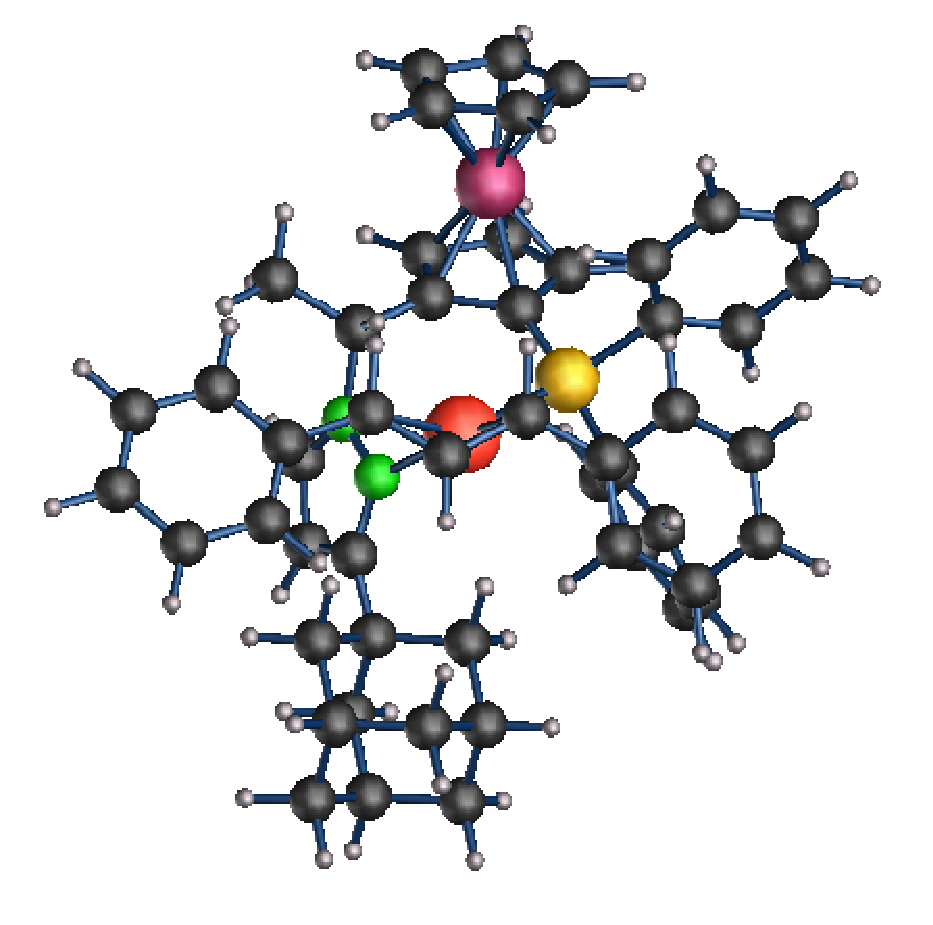
\includegraphics{Figs/big.eps}}
}
\date{\hrulefill\\Peter~E.~Bl\"ochl, IBM Zurich Research Laboratory\\(\today)}

\begin{document}          
%\maketitle   
%
\noindent            
\setcounter{page}{1}
%\footnote{The title picture shows the a chiral Pd complex with P,N ligands,
%  a highly enantio-selective catalyst for allylic amination \cite{Pdcat}.}
\newpage
\tableofcontents
%==========================================================================

%==========================================================================
\newpage
\section{The structure pre-optimization tool: paw\_preopt}
%==========================================================================

The paw\_preopt tool allows to perform a fast but inaccurate
structure pre-optimization based on force-field molecular dynamics. It
reads the structure input file (\verb'case.strc') and tries to find
bonds in the given structure using the covalent radii of the
atoms. Then it tries to find suitable parameterizations for the atoms
using the universal force field (UFF) \cite{UFF}. Bonds and force
field parameterizations can also be provided via the input files. Atoms
to be frozen can be specified. 

Using the parameterization it optimizes the geometry (currently) using
the conjugate gradient line search algorithm which is also used in
QM-MM coupling in the main simulation program. Atom positions after
optimization are printed to the protocol file and may be used as
starting point for a PAW simulation.

Atoms can be frozen during the optimization. No other constraints can
be applied. Freezing can either be done via the keywords
!PCNTL!FREEZEONLY and !PCNTL!MOVEONLY or via the keyword FREEZE=T in
the !ATOM block of the structure input file. The latter will be
ignored by the main PAW simulation program.

%==========================================================================
\subsection{Command}
%==========================================================================

The calling sequence is

\bigskip\fbox{{\tt paw\_preopt.x} {\it controlfile}}\bigskip

\noindent
where {\it controlfile} is the file name of the control input file for
the paw\_preopt tool. I recommend the extension ``.pcntl''.

%==========================================================================
\subsection{Example for the control input file}
%==========================================================================

\begin{verbatim}
!PCNTL
  !FILES
    !FILE ID='xyz' NAME='optimized.xyz' !END
  !END
  !GENERIC
    TRACE=F
    TOL=0.0001
    NSTEPS=10000
  !END
  !OUTPUT
     PRINTATOMS=T
     PRINTBONDS=T
     WARNFF=T
     XYZOUT=T
  !END
  !FREEZEONLY 
    COMMENT='This block has no effect as long as MOVEONLY is present.'
     !ATOM NAME='MO1' !END
     !ATOM PART='FE' !END
  !END
  !MOVEONLY
     !ATOM_OFF PART='H_nh' !END
     !ATOM NAME='N_nh41' !END
     !ATOM NAME='H_nh43' !END
     !ATOM NAME='H_nh44' !END
     !ATOM NAME='H_nh45' !END
  !END
!END
!EOB
\end{verbatim}

Please note that a keyword COMMENT is ignored by all PAW
programs. Thus it can be used to add comments to the input files.

%==========================================================================
%\newpage
\subsection{Argument description for the control input file}
%==========================================================================

%----------------------------------------------------------------------
\block{!PCNTL}
%----------------------------------------------------------------------
\brules{mandatory}
\bdescr{defines the operations done on the system; 
largely independent of the system}

%----------------------------------------------------------------------
\block{!PCNTL!GENERIC}
%----------------------------------------------------------------------
\brules{optional}
\bdescr{defines optimization parameters (and use of the trace)}

\mbax{\key{TRACE}
\vdescr{writes information on the calls of subroutines to standard output}
\vformat{logical} 
\vrules{optional}
\vdefault{F}}

\mbax{\key{TOL}
\vdescr{tolerance of the maximal component of the force on atoms in 
  the convergence cycles}
\vformat{real} 
\vrules{optional}
\vdefault{10$^{-4}$}}

\mbax{\key{NSTEPS}
\vdescr{maximal number of steps for the convergence. After that number
  the structure optimization is stopped no matter if the forces have
  become smaller than TOL. A statement on the convergence will be
  written to the protocol.}
\vformat{integer} 
\vrules{optional}
\vdefault{1000}}

%----------------------------------------------------------------------
\block{!PCNTL!FILES}
%----------------------------------------------------------------------
\brules{optional}
\bdescr{specifies the file names that deviate from the standard values}

%----------------------------------------------------------------------
\block{!PCNTL!FILES!FILE}
%----------------------------------------------------------------------
\brules{optional, multiple}
\bdescr{Specifies one file}

\mbax{\key{ID}
\vdescr{identifier for the file; options are: 
 \begin{description} 
 \item['PROT']protocol file \hfill\break Standard extension:'.pprot'
 \item['STRC'] The structure file as used by the simulation code. Used
   for the input structure. \hfill\break Standard extension:'.strc'
 \item['XYZ'] data file with the resulting optimized structure
   \hfill\break Standard extension:'.xyz'
 \end{description}
}
\vformat{character} 
\vrules{mandatory}
\vdefault{none}}

\mbax{\key{NAME}
\vdescr{filename. Can be the relative file name or an extension to the
  PAW ``root''. Standard output can be specified by NAME='stdout'
  and EXT=.false.}
\vformat{character} 
\vrules{mandatory}
\vdefault{none}}

\mbax{\key{EXT}
\vdescr{T: NAME specifies the extension only. F: full name}
\vformat{logical}
\vrules{optional}
\vdefault{F (false)}}

%----------------------------------------------------------------------
\block{!PCNTL!OUTPUT}
%----------------------------------------------------------------------
\brules{optional}
\bdescr{specifies which information should be written to the protocol}

\mbax{\key{PRINTATOMS}
\vdescr{information on the used atom parameterization and freezing is
  written to the protocol}
\vformat{logical} 
\vrules{optional}
\vdefault{T}}

\mbax{\key{PRINTBONDS}
\vdescr{information on the used bonds is
  written to the protocol}
\vformat{logical} 
\vrules{optional}
\vdefault{T}}

\mbax{\key{WARNFF}
\vdescr{paw\_preopt tries to find best-suiting force fields for the
  atoms. However, in some cases it cannot decide which parameterization
  will be the best. If T in these cases a warning will be printed to
  the protocol.}
\vformat{logical} 
\vrules{optional}
\vdefault{T}}

\mbax{\key{XYZOUT}
\vdescr{should an xyz-file of the resulting structure be created?}
\vformat{logical} 
\vrules{optional}
\vdefault{T}}


%----------------------------------------------------------------------
\block{!PCNTL!FREEZEONLY}
%----------------------------------------------------------------------
\brules{optional, not used if !PCNTL!MOVEONLY is present}
\bdescr{sets freezing of all atoms but those specified in this block
  to false. May be overwritten for single atoms by !STRC!ATOM:FREEZE}

\mbax{\key{NAME}
\vdescr{specifies an atom name}
\vformat{character} 
\vrules{optional, multiple}
\vdefault{none}}

\mbax{\key{PART}
\vdescr{Specifies a part of an atom name. All atoms containing this
  string are used. Case is ignored.}
\vformat{character} 
\vrules{optional, multiple}
\vdefault{none}}

%----------------------------------------------------------------------
\block{!PCNTL!MOVEONLY}
%----------------------------------------------------------------------
\brules{optional, overwrites !PCNTL!FREEZEONLY}
\bdescr{sets freezing of all atoms but those specified in this block
  to true. May be overwritten for single atoms by !STRC!ATOM:FREEZE}

\mbax{\key{NAME}
\vdescr{specifies an atom name}
\vformat{character} 
\vrules{optional, multiple}
\vdefault{none}}

\mbax{\key{PART}
\vdescr{Specifies a part of an atom name. All atoms containing this
  string are used. Case is ignored.}
\vformat{character} 
\vrules{optional, multiple}
\vdefault{none}}

%==========================================================================
%\newpage
\subsection{Argument description for the structure input file}
%==========================================================================

The atomic structure is read from a structure input file which has the
same syntax as for the main simulation code. However, a few keywords
are used which are ignored by the main simulation code. The keyword
!STRC!GENERIC:LUNIT is mandatory.

%----------------------------------------------------------------------
\block{!STRC!ATOM}
%----------------------------------------------------------------------
\brules{mandatory,multiple}
\bdescr{usage is same as in the main simulation code. Keywords R, SP
  and NAME are used. Additional keywords are:}

\mbax{\key{FFTYPE}
\vdescr{Force field type used for this atom. This keyword can be used
  to overwrite the suggestion of the program. Possible force fields
  can be found in section~\ref{uff} on page~\pageref{uff}.}
\vformat{character} 
\vrules{optional}
\vdefault{depending on the atom type and the number of bonds to that atom}}

\mbax{\key{FREEZE}
\vdescr{freeze this atom}
\vformat{logical} 
\vrules{optional}
\vdefault{F}}

%----------------------------------------------------------------------
\block{!STRC!BOND}
%----------------------------------------------------------------------
\brules{optional,multiple}
\bdescr{Overwrite the suggestion of the program for bonds between the
  atoms. Not yet implemented.}

%==========================================================================
\newpage
\section{The Universal Force Field (UFF) \cite{UFF} \label{uff}}
%==========================================================================

UFF is used in the QM-MM coupling and in the pre-optimization tool
paw\_preopt. It has been published in \cite{UFF}. Parts of that paper
most important for calculations are given here. 

The original UFF has 126 atom types, however in the CP-PAW
implementation there are currently 141 and occasionally some more may
be added. In case of uncertainty have a look into the code: subroutine
\texttt{UFFTABLE\_INI} in the file \texttt{paw\_classical.f}. A
five-character mnemonic label is used to describe the atom types. The
first two characters correspond to the chemical symbol; an underscore
appears in the second column if the symbol has one letter. The third
column describes the hybridization or geometry: 1=linear, 2=trigonal,
R=resonant, 3=tetrahedral, 4=square planar, 5=trigonal bipyramidal,
6=octahedral. Thus N\_3 is tetrahedral nitrogen, while Rh6 is
octahedral rhodium. The fourth and fifth columns are used as indicators
for alternate parameters such as formal oxidation state: Rh6+3
indicates an octahedral rhodium formally in the +3 oxidation
state. H\_\_\_B indicates a bridging hydrogen as in B$_2$H$_6$.  Some
parameters of the implementation of UFF in the CP-PAW code are given
in the following table. \verb'bond' is the bond radius in \AA{} and
\verb'angle' the bond angle in degrees.

\scriptsize
\begin{verbatim}
FFTYPE  BOND  ANGLE      FFTYPE  BOND  ANGLE
H_     0.354  180.000    AG1+1  1.386  180.000
H___B  0.460   83.500 	 CD3+2  1.403  109.471
HE4+4  0.849   90.000 	 IN3+3  1.459  109.471
LI     1.336  180.000 	 SN3    1.398  109.471
BE3+2  1.074  109.471 	 SB3+3  1.407   91.600
B_3    0.838  109.471 	 TE3+2  1.386   90.250
B_2    0.828  120.000 	 I_     1.382  180.000
C_3    0.757  109.471 	 XE4+4  1.267   90.000
C_R    0.729  120.000 	 CS     2.570  180.000
C_2    0.732  120.000 	 BA6+2  2.277   90.000
C_1    0.706  180.000 	 LA3+3  1.943  109.471
N_3    0.700  106.700 	 CE6+3  1.841   90.000
N_R    0.699  120.000 	 PR6+3  1.823   90.000
N_2    0.685  111.300 	 ND6+3  1.816   90.000
N_1    0.656  180.000 	 PM6+3  1.801   90.000
O_3    0.658  104.510 	 SM6+3  1.780   90.000
O_3_Z  0.528  145.500 	 EU6+3  1.771   90.000
O_R    0.680  110.300 	 GD6+3  1.735   90.000
O_2    0.634  120.000 	 TB6+3  1.732   90.000
O_1    0.639  180.000 	 DY6+3  1.710   90.000
F_     0.668  180.000 	 HO6+3  1.696   90.000
NE4+4  0.920   90.000 	 ER6+3  1.673   90.000
NA     1.539  180.000 	 TM6+3  1.660   90.000
MG3+2  1.421  109.471 	 YB6+3  1.637   90.000
AL3    1.244  109.471 	 LU6+3  1.671   90.000
SI3    1.117  109.471 	 HF3+4  1.611  109.471
P_3+3  1.101   93.800 	 TA3+5  1.511  109.471
P_3+5  1.056  109.471 	 W_6+6  1.392   90.000
P_3+Q  1.056  109.471 	 W_3+4  1.526  109.471
S_3+2  1.064   92.100 	 W_3+6  1.380  109.471
S_3+4  1.049  103.200 	 RE6+5  1.372   90.000
S_3+6  1.027  109.471 	 RE3+7  1.314  109.471
S_R    1.077   92.200 	 OS6+6  1.372   90.000
S_2    0.854  120.000 	 IR6+3  1.371   90.000
CL     1.044  180.000 	 PT4+2  1.364   90.000
AR4+4  1.032   90.000 	 AU4+3  1.262   90.000
K_     1.953  180.000 	 HG1+2  1.340  180.000
CA6+2  1.761   90.000 	 TL3+3  1.518  120.000
SC3+3  1.513  109.471 	 PB3    1.459  109.471
TI3+4  1.412  109.471 	 BI3+3  1.512   90.000
TI6+4  1.412   90.000 	 PO3+2  1.500   90.000
V_3+5  1.402  109.471 	 AT     1.545  180.000
CR6+3  1.345   90.000 	 RN4+4  1.420   90.000
MN6+2  1.382   90.000 	 FR     2.880  180.000
FE3+2  1.412  109.470 	 RA6+2  2.512   90.000
FE6+2  1.335   90.000 	 AC6+3  1.983   90.000
CO6+3  1.241   90.000 	 TH6+4  1.721   90.000
NI4+2  1.164   90.000 	 PA6+4  1.711   90.000
CU3+1  1.302  109.471 	 U_6+4  1.684   90.000
ZN3+2  1.193  109.471 	 NP6+4  1.666   90.000
GA3+3  1.260  109.471 	 PU6+4  1.657   90.000
GE3    1.197  109.471 	 AM6+4  1.660   90.000
AS3+3  1.211   92.100 	 CM6+3  1.801   90.000
SE3+2  1.190   90.600 	 BK6+3  1.761   90.000
BR     1.192  180.000 	 CF6+3  1.750   90.000
KR4+4  1.147   90.000 	 ES6+3  1.724   90.000
RB     2.260  180.000 	 FM6+3  1.712   90.000
SR6+2  2.052   90.000 	 MD6+3  1.689   90.000
Y_3+3  1.698  109.471 	 NO6+3  1.679   90.000
ZR3+4  1.564  109.471 	 LW6+3  1.698   90.000
NB3+5  1.473  109.471 	 CPR    0.551   90.000
MO6+6  1.467   90.000 	 CPR_B  0.340   90.000
MO3+6  1.484  109.471 	 CIR    0.616   90.000
TC6+5  1.322   90.000 	 PIR    0.616   90.000
RU6+2  1.478   90.000 
RH6+3  1.332   90.000 
PD4+2  1.338   90.000 
\end{verbatim}
\normalsize

%====================================================================
\newpage
\begin{thebibliography}{99}
%0
\bibitem{Pdcat} ``First-Principles Investigation of Enantioselective
  Catalysis: Asymmetric Allylic Amination with Pd Complexes Bearing P,
  N Ligands'', P.E. Bl\"ochl and A. Togni, Organometallics {\bf 15},
  4125 (1996).
%1
\bibitem{PAW}``Projector Augmented Wave Method'', P.E. Bl\"ochl, Phys.
  Rev. B {\bf 50}, 17953 (1994).
%2
\bibitem{KohnSham} ``Inhomogeneous Electron Gas'', P.~Hohenberg and
  W.~Kohn, Phys. Rev.{\bf 136} B 864 (1964); ``Selfconsistent Equations
  including exchange and Correlation Effects'', W.~Kohn and L.J.~Sham,
  Phys. Rev. {\bf 140}, A1133 (1965)
%3
\bibitem{DFTBenchmarks} ``Density Functional Thermochemistry~II. The
  effect of the Perdew-Wang Generalized-Gradient Correlation
  Correction'', A.D.~Becke, J. Chem. Phys. {\bf 97}, 9173 (1992),
  ``Basis-set-free local density-functional calculations of geometries
  of polyatiomic molecules'', R.M.~Dickson and A.D.~Becke,
  J. Chem. Phys. {\bf 99}, 3898 (1993).
%4
\bibitem{CP}``Unified Approach for Molecular Dynamics and Density
  Functional Theory'', R.~Car and M.~Parrinello, Phys. Rev. Lett. {\bf
    55}, 2471 (1985).
%5
\bibitem{CP2} ``The Unified Approach for Molecular Dynamics and
  Density Functional Theory'', R. Car and M. Parrinello, in {\it
    Simple molecular systems at very high density} ed. A. Polian et
  al. (Plenum, New York, 1989) p455-476.
%6
\bibitem{Pastore}G.~Pastore, E.~Smargiassi and F.~Buda, Phys. Rev. A
  {\bf 44}, 6334 (1991).
%7
\bibitem{Madden} ``Molecular Dynamics without Effective Potentials via
  the Car-Parrinello Approach'', D.K.~Kremler and P.A.~Madden, Mol.
  Phys. {\bf 70}, 921 (1990).
%8
\bibitem{Decouple}``Electrostatic decoupling of plane wave expanded
  densities and derived atomic point charges'', P.E.~Bl\"ochl, J.
  Chem. Phys. {\bf 103}, 7422 (1995).
%9
\bibitem{MPI} Message Passing Interface. Software for interprocessor
  communication on parallel computers. See
  ``http://www.osc.edu/Lam/lam.html\#MPI'' for more information.
%10
\bibitem{ESSL} Engineering and Scientific Subroutine Library is a
  product of IBM. See
  ``http://direct.boulder.ibm.com/rsdirect/us/software/essl.htm'' for
  more information.
%0
\bibitem{IRC} ``A Formulation of the Reaction Coordinate'' J. Phys.
  Chem. {\bf 74}, 4161 (1970); ``The Path of Chemical Reactions -- The
  IRC Approach'' Acc. Chem. Res. {\bf 14}, 363 (1981).
%11
\bibitem{Constants}``The Fundamental Physical Constants'' E.R.~Cohen
  and B.N. Taylor, Physics Today {\bf 49} (Buyers Guide), 9 (1996) and
  references therein.
%12
\bibitem{Dataexplorer} The IBM Visualization Dataexplorer is a
  general-purpose software package for data visualization and
  analysis. See ``http://www.opendx.org/'' for information. It is now
  an open source project and publically available at no cost.
%13
\bibitem{XMGR}XMGR is an XY plotting tool written by 
  Paul~J.~Turner. The development is currently being continued by a group of
  volunteers.  For information on how to obtain access, see
  ``http://plasma-gate.weizmann.ac.il/Xmgr/''.
%14
\bibitem{Cerius2} Cerius$^2$ is a product of Molecular Simulations
  Inc. See ``http://www.msi.com/info/products/Cerius2.html'' for more
  information.
%15
\bibitem{PerdewZunger} ``Self-interaction correction to
  density-functional approximations for many-electron
  systems'', J.P.~Perdew and A.~Zunger, Phys. Rev. B {\bf 23}, 5048 (1981).
%16
\bibitem{CeperleyAlder} ``Ground State of the Electron Gas by a
  Stochastic Method'' D.M.~Ceperley and B.J.~Alder, Phys. Rev.
  Lett. {\bf 45}, 566 (1980).
%17
\bibitem{GGA91}``Atoms, Molecules, Solids, and Surfaces: Applications
  of the Generalized Gradient Approximation for Exchange and
  Correlation'', J.P.~Perdew, J. A. Chevary, S.H.~Vosko, K.A.~Jackson,
  M.R.~Pederson, D.J.~Singh and C.~Fiolhais, Phys. Rev. B, {\bf 46},
  6671 (1992-I).
%17
\bibitem{PW91L} ``Accurate and simple analytic representation of the
  electron gas correlation energy'', J.P.~Perdew and Y.~Wang,
  Phys. Rev.B {\bf 45}, 13244 (1992-I)
%18
\bibitem{Becke88}``Density Functional Exchange Energy Approxiamtion
  with Correct Asymptotic Behavior'', A.D.~Becke, J. Chem. Phys.{\bf
    96}, 2155 (1992).
%19
\bibitem{Perdew86} ``Density-Functional Approximations for the
  Correlation Energy of the Inhomogeneous Electron Gas'', J.P.~Perdew,
  Phys. Rev. B {\bf 33}, 8822 (1986)).
%20
\bibitem{PBE}``Generalized Gradient Approximation Made Simple'',
  J.P.~Perdew, K.~Burke and M.~Ernzerhof, Phys. Rev. Lett. {\bf 77},
  3865 (1996).
%21
\bibitem{Verlet}``Practical Algorithms for Dynamic Simulations'',
  H.J.C.~Berendsen and W.F.~van Gunsteren, Varenna Notes (1985), p43.
%22
\bibitem{Acceleration}``Acceleration schemes for ab-initio molecular
  dynamics simulations and electronic structure calculations''
  F.~Tassone, F.~Mauri and R.~Car, Phys. Rev. B {\bf 50}, 10561
  (1994-I)
%23
\bibitem{Adiabaticity}``Adiabaticity in first-principles molecular
  dynamics'', P.E.~Bl\"ochl and M.~Parrinello, Phys. Rev. B {\bf 45},
  9413 (1992).
%24
\bibitem{Nose}``A unified formulation of the constant temperature
  molecular dynamics methods'', S.~Nos\'e, J. Chem. Phys. {\bf 81}, 511
  (1984); ``A molecular dynamics method for simulation in the
  canonical ensemble'', S.~Nos\'e, Mol.  Phys. {\bf 52}, 255 (1984),
  ``Canonical Dynamics: Equilibrium phase-space distributions'', W.G.
  Hoover, Phys. Rev. A {\bf 31}, 1695 (1985).
%25
\bibitem{Constraints} ``Numerical Integration of the Cartesian
  Equations of Motion of Systems with Constraints: Molecular
  Dynamics of n-Alkanes'' J.-P.~Ryckaert, G.~Cicotti and H.J.C.~Berendsen,
  J. Comp. Phys. {\bf 23}, 327 (1977).
%26
\bibitem{HinSi} ``First-Principles Calculations of Diffusion Constants:
  Hydrogen in Silicon'', P.E.~Bl\"ochl, C.G.~Van~de~Walle and
  S.T.~Pantelides, Phys. Rev. Lett. {\bf 64}, 1401 (1990). 
%27
\bibitem{UFF} ``UFF, a fully periodic table force field for molecular
  mechanics and molecular dynamics simulations'' A.K.~Rappe,
  C.J.~Casewit, K.S.~Colwell, W.A.~Goddard~III, and W.M.~Skiff,
  J. Am. Chem. Soc. {\bf 114}, 10024 (1992).
%28
\bibitem{FreeSoftwareFoundation} For information of software from the
  free software foundation, see ``http://www.gnu.ai.mit.edu/''
%??
\bibitem{LDA+U}``Band Theory and Mott Insulators: Hubbard U instead of
  Stoner I'', V.I.~Anisimov, J.~Zaanen and 
O.K.~Andersen, Phys. Rev. B {\bf 44}, 943 (1991).
%
\bibitem{MPEGPLAY}``http://www.geom.umn.edu/software/mpeg\_play/''
%
\bibitem{MPEGENCODE} ``http://www.imag.fr/Multimedia/archives/unix.html''
%
\bibitem{Beckethermochemistry}``Density Functional Thermochemistry I:
  The effect of exchange-only gradient correction'', A.D. Becke,
  J.chem. Phys. {\bf 96}, 2155 (1992); ``Density Functional
  Thermochemistry II: The effect of Perdew Wang generalized-gradient
  correlation correction'', A.D. Becke, J.chem. Phys. {\bf 97}, 9173
  (1992);
%
\bibitem{Pople} ``Gaussian-1 theory: A general procedure for prediction
  of molecular energies'' J.A. Pople, M. Head-Gordon and D.J. Fox,
  J. Chem. Phys. {\bf 90}, 5622 (1989); ``Gaussian-1 theory of
  molecular energies for second-row compounds'' L.A. Curtiss,
  C. Jones, G.W. trucks and K. Raghavachari,
  J. Chem. Phys. {\bf 93}, 2537(1990)
\end{thebibliography}
\end{document}
\bye
%====================================================================
